\documentclass[BCOR=12mm,DIV11,titlepage,a4paper,oneside]{scrbook}

%Paket für deutsche Silbentrennung etc.
\usepackage{ngerman}

%Paket für Zeichenkodierung, entspricht UTF-8
\usepackage[utf8x]{inputenc}

%Paket das die Ausgabefonts definiert
\usepackage[T1]{fontenc}

%Paket für Sonderzeichen wir RightsReserved
\usepackage{textcomp}

%Euro-Symbol
\usepackage[right]{eurosym}

%Paket für das Einbinden von Grafiken über die figure-Umgebung
\usepackage{graphicx}

%Paket zum Ändern der Kopf- und Fußzeile
\usepackage{fancyhdr}
%Benutzt das Paket für eigenen Seitenstil
\pagestyle{fancy} 
%Erzeugt eine Linie in der Kopfzeile (lässt sich mit 0.0pt ausblenden)
\renewcommand*{\headrulewidth}{0.4pt} 
\fancyhf{}
\fancyhead[EC,OC]{\thepage}
% \fancyhead[EL]{\leftmark} 
% \fancyhead[OR]{\rightmark} 
% \fancyhead[ER,OL]{\thepage}
\renewcommand{\sectionmark}[1]{ 
\markboth{\thechapter{} #1}{\thechapter{} #1} 
}
%Ändert die Seitennummerierung beim Inhaltsverzeichnis mit eigenem Stil
\renewcommand*{\indexpagestyle}{fancy}
%Verhindert die Seitennummerierung auf den Part-Seiten
\renewcommand*{\partpagestyle}{empty}
%Ändert die Seitennummerierung bei Chapter mit eigenem Stil
\renewcommand*{\chapterpagestyle}{fancy}

%Abbildungsnummerierung ändern (abhängig von chapter, z.B. Abbildung 1.1)
\renewcommand*{\thefigure}{\thechapter.\arabic{figure}}
%Tabellennummerierung ändern (abhängig von chapter, z.B. Tabelle 1.1)
\renewcommand*{\thetable}{\thechapter.\arabic{table}}

%Paket, um ein Glossar/Abkürzungsverzeichnis anzulegen
\usepackage{nomencl}
\let\abbrev\nomenclature
%Der Name wird in Glossar geändert
\renewcommand{\nomname}{Glossar (optional)}
%Definiert die Aufteilung im Glossar zwischen Begriffen und Erläuterung
\setlength{\nomlabelwidth}{.25\hsize}
%Definiert die Punktelinien im Glossar
\renewcommand{\nomlabel}[1]{#1 \dotfill}
\setlength{\nomitemsep}{-\parsep}
%Veranlasst die Erstellung des Glossars
\makenomenclature

%Einrückungen nach Absätzen und Grafiken verhindern
\setlength{\parindent}{0pt}



%Verhindern, dass eine neue Seite für ein einzelnes Wort/Zeile verwendet wird
\clubpenalty = 10000 % schliesst Schusterjungen aus 
\widowpenalty = 10000 % schliesst Hurenkinder aus (keine Beleidigung, sondern wirklich ein Fachbegriff)

%Paket für ein deutsches Literaturverzeichnis
\usepackage[authoryear,square]{natbib}
\bibliographystyle{natdin}
% \setlength\bibhang{30pt}

%Paket für die Verwendung von URLs durch den Befehl \url{}
\usepackage{url}

%Paket für Zeilenabstand (onehalfspace, singlespace)
\usepackage{setspace}

%Paket zur Erzeugung von Anführungszeichen durch \enquote{Text}
\usepackage[ngerman]{babel}
\usepackage[babel, german=quotes]{csquotes}

%Paket für farbigen Text
%black,white,green,red,blue,yellow,cyan,magenta
\usepackage{color}
%Farbige Tabellen
\usepackage{colortbl}

%Rotation von Gleitobjekten (Grafiken, Trabellen, etc.)
\usepackage{rotating}

%Rotation von einzelnen Seiten begin{landscape}
\usepackage{lscape}

%Paket für farbigen Hintergrund für Verbatim-Umgebung (Quelltext-Umgebung)
\usepackage{fancyvrb}
\usepackage{verbatim,moreverb}
%Grauton für Quelltext-Umgebung definieren 80% Grau
\definecolor{sourcegray}{gray}{.80}
%Paket für Quelltext-Umgebung
\usepackage{listings}
%Alternative Quelltext-Umgebung
%\lstset{numbers=left, 
%	numberstyle=\tiny, 
%	numbersep=5pt,
%	language=Java,
%	breaklines=true,
%	breakautoindent=true,
%	postbreak=\space,
%	tabsize=2,
%	frame=tlrb,
%	basicstyle=\ttfamily\footnotesize}

%Paket für Positionierung der Objekte ohne Float (Verwendungsbsp.: \begin{figure}[H])
%\usepackage{here}
%Alternatives Paket für here.sty
\usepackage{float}

%DRAFT als Wasserzeichen im Hintergrund
% \usepackage{draftwatermark} 
% \SetWatermarkAngle{60}
% \SetWatermarkScale{5.0}

%Für lange Tabellen
\usepackage{longtable,array,supertabular}

%Für rowspan in Tabellen
\usepackage{multirow}

%Behält die Schriftgröße der Überschrift normal, wenn z.B. die Schriftgröße in einer Tabelle verändert wird
\addtokomafont{caption}{\normalsize} 

%Paket um PDF Seiten einzubinden
\usepackage{pdfpages}

%Paket zur Erzeugung von Hyperrefs und PDF Informationen
\usepackage[pdftex,plainpages=false,pdfpagelabels,
            pdftitle={title},
            pdfauthor={name}
            ]{hyperref}
%Farben für Links
%Farbige Ränder bei false und farbige Texte bei true
\hypersetup{colorlinks=true,citecolor=black,filecolor=black,linkcolor=black,urlcolor=black}

%Zwei Verzeichnisse für Inhalt und Anhang
\usepackage{appendix}
% \usepackage{minitoc} 
% \nomtcrule
% \renewcommand{\mtctitle}{Anhangsverzeichnis}
% \setlength{\mtcindent}{0pt} 

\begin{document}

%=== Einleitung ======================================================
\frontmatter 
\setcounter{page}{3}
\pagenumbering{arabic}



\begin{titlepage}

%Logo der technischen Hochschule Köln
\begin{center}
\begin{figure*}[!ht]
	\flushright
		
\includegraphics[width=.2\textwidth]{images/logo.pdf}
		
\includegraphics[width=\textwidth]{images/balken.png}
\end{figure*}

\vspace{1.5cm}


% Titel
\begin{rmfamily}
\begin{huge}
\textbf{Brute Force Angriff auf einem parallelem, verteilten System}\\	
\end{huge}
\vspace{0.5cm}
\end{rmfamily}

\vspace{1.6cm}

\begin{LARGE}
\begin{scshape}
Dokumentation Architektur verteilter Systeme\\[0.8em]
\end{scshape}
\end{LARGE}

%ausgearbeitet von...
\begin{large}
ausgearbeitet von\\ 
\vspace{0.2cm}
\begin{LARGE}
Sebastian Domke\\
Pascal Schönthier\\
Dennis Jaeger\\
\end{LARGE}
\end{large}

\vspace{1.0cm}

%vorgelegt an der...
\begin{large} 
\vspace{0.2cm}
\begin{scshape}
TH Köln\\
Campus Gummersbach\\
Fakultät für Informatik
\end{scshape}
\end{large}

\vspace{0.4cm}

%im Studiengang...
\begin{large}
im Studiengang\\ 
\vspace{0.2cm}
\textsc{Computer Science Master \\
Software Engineering}
\end{large}


\vspace{1.0cm}

\begin{tabular}{rl}
	vorgelegt bei:  &  Prof. Dr. Lutz Köhler\\
       					&  \small TH Köln \\[1.0em]
\end{tabular}

\vspace{1.6cm}

%Ort, Monat der Abgabe
\begin{large}
Gummersbach, {\today}
\end{large}
\end{center}

\vspace{2.0cm}

\newpage
\thispagestyle{empty}

\end{titlepage}

\singlespacing

%Einbinden eines Vorwortes
\chapter*{Kurzbeschreibung}
\addcontentsline{toc}{chapter}{Vorwort}

Diese Dokumentation wird im Rahmen des Moduls \textbf{Architektur verteilter Systeme} im Studiengang Computer Science Master, Fachrichtung Software Engineering, an der technischen Hochschule Köln am Campus Gummersbach erstellt. \\

Das Ziel ist die prototypische Implementierung eines Brute Force Algorithmus innerhalb einer verteilten Architektur.\\
Mit Hilfe des Brute Force-Angriffs soll ein vordefiniertes Passwort entschlüsselt werden. \\
Um dies zu realisieren, werden mögliche Passwort-Hash-Kombinationen berechnet und mit einem Ziel-Hash verglichen. Sobald ein berechneter Hash mit dem Ziel-Hash übereinstimmt, ist der Angriff erfolgreich abgeschlossen. \\

Die Implementierung soll in der von Apple\textsuperscript{\textcopyright} entwickelten Programmiersprache Swift umgesetzt und den allgemeinen Prinzipien eines verteilten Systems gerecht werden. 

%Für Anhangsverzeichnis
% \dominitoc

\tableofcontents
\onehalfspacing

%=== Hauptteil =======================================================
\mainmatter
\setcounter{page}{4}

\setcounter{table}{1}
\setcounter{figure}{1}
	%!TEX root = ../VorlageBA.tex
\chapter{Motivation und Grundlagen}

\section{Grundlagen}
\label{grundlagen}
Zu Beginn der Grundlagen wird eine generische Definition eines \emph{verteilten Systems} genannt:
\begin{quotation}
	\textit{\enquote{Ein verteiltes System ist eine Ansammlung unabhängiger Computer, die den Benutzern wie ein einzelnes kohärentes System erscheinen.}} \citep{tanenbaum}
\end{quotation}




 
	
	
\setcounter{table}{1}
\setcounter{figure}{1}
	\chapter{Grundlagen des verteilten Systems}
\label{Grundlagen}
Dieses Kapitel bietet Informationen zur verwendeten Hard- und Software. Damit werden die Umstände, unter denen das Projekt durchgeführt wird, verdeutlicht. Außerdem wird die Reproduzierbarkeit und damit der wissenschaftliche Anspruch an das Projekt realisiert. 

\section{Hardware}
\label{Hardware}
Das verteilte System wird auf einem Mac-Cluster implementiert, das von der Hochschule zur Verfügung gestellt wird. Es kann auf 10 Rechner zugegriffen werden, die mit \emph{pip02} bis \emph{pip11} gekennzeichnet sind. Auf allen Rechnern ist (Stand 09.07.2016) aktuellste Version des Betriebssystems El Capitain und der Entwicklungsumgebung Xcode installiert. Details zu den Softwareversionen sind in Kapitel \ref{softwarebasis} zu finden. \\
In der folgenden Liste sind die Details zu den einzelnen Rechnern zu aufgeführt:

\begin{itemize}
	\item\textbf{pip02-pip05: Mac Pro (Anfang 2008)}
	\item[]Seriennummer: CK8250EUXYL
	\item[]Prozessor: 	2 x 2,8 GHz Quad-Core Intel Xeon 
	\item[]RAM: 8 GB 800 MHz DDR2 FB-DIMM
	\item[]Grafikkarte: 	NVIDIA GeForce 8800 GT (512MB)
	\item[]OS 10.11.5 El Capitain
	\item[]Xcode 7.3, Swift 2.1.1 
	\item\textbf{pip06-pip11: Mac Pro (Anfang 2009)}
	\item[] Seriennummer: CK92608B20H
	\item[]Prozessor: 2 x 2,26 GHz Quad-Core Intel Xeon 
	\item[]RAM: 8 GB 1066 MHz DDR3 ECC
	\item[]Grafikkarte: 	NVIDIA GeForce GT 120 (512MB)
	\item[] OS 10.11.5 El Capitain
	\item[] Xcode 7.3, Swift 2.1.1
	\end{itemize}

Zur Netzverbindung wird ein Switch des Herstellers \emph{Netgear} eingesetzt. Die Modellbezeichnung lautet \emph{Netgear GS116}. Der Switch hat 16 Ports und unterstützt bis zu 1024 Megabit/s (Gigabit-LAN).

\section{Software}
\label{softwarebasis}
Da Rechner des Herstellers Apple eingesetzt werden, sind die Programmiersprachen \emph{Objective C} oder \emph{Swift} effizient einsetzbar, da Apple diese vorrangig unterstützt. Das eingesetzte Betriebssystem Mac OS X 10.11.2 (El Capitain) und die native Entwicklungsumgebung Xcode 7.2 weisen eine hohe Kompatibilität zu den genannten Programmiersprachen auf. \\
Da die Programmiersprache \emph{Swift} seit Version 2.0 quelloffen angeboten wird\footnote{\url{https://github.com/apple/swift}} und zudem die aktuellere der beiden genannten Sprachen ist, möchte das Projektteam primär auf Swift zurückgreifen. Da aktuell der Einsatz von Objective C noch Bestandteil von Swift ist, werden beide genannten Programmiersprachen zum Einsatz kommen. Ziel ist es aber, möglichst nur auf Swift zurückzugreifen und Objective C nur dann einzusetzen, wenn keine andere Möglichkeit besteht. \\
\subsection{Versionsverwaltung}
Zur Versionierung des Programmcodes und zum vereinfachtem dezentralen Entwickeln wird die Programmcode-Plattform \url{www.github.com} eingesetzt. Die auf dem Versions-verwaltungs-System \emph{Git} basierende Plattform ermöglicht ein flexibles und kollaboratives Arbeiten am Projekt sowie der Dokumentation. \\
Zum Abschluss wird in Kapitel \ref{fazit} ein Verweis zum Projekt auf \emph{Github} bereitgestellt. 
\subsection{Frameworks}
Damit im Projekt weitere Frameworks mit wenig Aufwand eingesetzt werden können, hat das Projektteam sich entschieden \emph{Carthage}\footnote{\url{https://github.com/Carthage/Carthage}} einzusetzen. Carthage ist ein \enquote{einfacher, dezentraler Dependency-Manager} und wird quelloffen zur Verfügung gestellt. Durch die Auflösung von Abhängigkeiten, beispielsweise von bestimmten Frameworks, wird das asynchrone und dezentrale Entwickeln weiter optimiert. \\
Als alternativer Dependency-Manager hätte sich das Werkzeug \emph{CocoaPods}\footnote{\url{https://github.com/CocoaPods/CocoaPods}} angeboten. Einer der großen Unterschiede in der Arbeitsweise der beiden Werkzeuge liegt in der Verwaltung der Dependencies. Während CocoaPods auf eine zentrale Verwaltung setzt, werden die Abhängigkeiten bei Carthage dezentral verwaltet. Durch die dezentrale Verwaltung wird unser Primärziel, das effektive kollaborative Arbeiten, besser abgedeckt. Zudem wird Carthage leichtgewichtiger im Projekt, als es bei CocoaPods der Fall wäre. Dadurch entsteht eine weniger starke Abhängigkeit. Aus den genannten Gründen fiel die Wahl auf die Verwendung von Carthage. \\
Zudem wird die Plattform \emph{Node.JS} benutzt, um einen Kommunikationsserver zur Verfügung zu stellen. Weitere Informationen dazu sind in Kapitel \ref{Konzeption} zu finden. 


%======================================================================
%======================================================================
% Eintraege ins Glossar
\nomenclature{BruteForce-Angriff}{Entschlüsselung eines unbekannten Passwortes, indem alle möglichen Zeichenkombinationen durchprobiert werden, bis das korrekte Passwort ermittelt ist.\vspace{4mm}}

\nomenclature{Dictionary-Angriff}{Effiziente Methode zum Entschlüsseln eines unbekannten Passwortes. Basis dazu ist ein Wörterbuch mit häufig benutzten Passwörtern, die nach einer festgelegten Strategie durchprobiert werden.\vspace{4mm}}
\nomenclature{Master}{Instanz innerhalb des verteilten Systems, welche für die Verteilung der anfallenden Tätigkeiten verantwortlich ist.\vspace{4mm}}

\nomenclature{Worker}{Instanz innerhalb des verteilten Systems, welche für die Bearbeitung der anfallenden Tätigkeiten verantwortlich ist.\vspace{4mm}}


\nomenclature{Provider}{Synonym für den \emph{Master}.\vspace{4mm}}




 
	
	\setcounter{table}{1}
\setcounter{figure}{1}
	\chapter{Konzeption}
\label{Konzeption}
Nachfolgend wird die Konzeption des Projekts beschrieben. 
Die Kommunikation wird nachrichtenbasiert umgesetzt. Dies bedeutet, dass die Komponenten des verteilten Systems kommunizieren, indem sich sich Nachrichten zusenden. Die Steuerung der Kommunikation wird primär von den als Master 
(siehe \ref{glossar}) ausgewählten Komponenten umgesetzt. Als Provider wird ein an das Projekt angepasster Webserver eingesetzt. Die Verbindung der einzelnen Komponenten zueinander geschieht über WebSockets. \\


\section{Brute Force-Algorithmus}
\label{ideeBruteForce}
Primäres Ziel des Projektes ist das Entschlüsseln eines vorgegebenen Passwortes. Das zu entschlüsselnde Passwort wird vor der Berechnung vom Benutzer eingegeben. Das eingetragene Passwort wird dann durch eine Hashfunktion geleitet. Der erzeugte Hash wird gespeichert und dient als Zielbedingung der folgenden Berechnung. \\
Nun beginnt der eigentliche Angriff. Zu Beginn wird eine sogenannte \enquote{Dictionary-Attack} vorgenommen. Dies bedeutet, dass ein Wörterbuch mit häufig genutzten Passwörtern als Basis des Angriffs genutzt wird. Die eingetragenen Passwörter werden ebenfalls der Reihe nach gehasht und der berechnete Hash mit dem Zielhash verglichen. \\
 Durch die vorangestellte Attacke auf Basis von häufig benutzten Passwörtern wird die Effizienz des verteilten Systems verbessert. Der folgende Auszug aus der Passwortliste  verdeutlicht das Prinzip eines Dictionaries. \\
 \newpage
\texttt{Dictionary:}
\begin{lstlisting}[basicstyle=\ttfamily,numbers=left,numberstyle=\footnotesize\ttfamily,backgroundcolor=\color{sourcegray}]
	LOVE123
	LOVEME1
	Lamont1
	Leasowes2
	Lemon123
	Liberty
	Lindsay
	Lizard
	Love21
	MASTER
	MORIAH07
	MOSS18
	Madeline
	Margaret
	Master
	Matthew
	Maxwell
	Mellon
	Merlot
	Metallic
	Michael
\end{lstlisting}



Bleibt die Dictionary-Attack erfolglos, wir der BruteForce-Angriff durchgeführt. \\
Die erste Idee war es, dass der steuernde Rechner alle möglichen Passwörter berechnet und in einem Array ablegen wird. Dabei sollten die Passwörter eine statische Länge besitzen. Das Muster der möglichen Passwörter sollte wie folgt aufgebaut werden: \\

\texttt{Muster der zu berechnenden Passwörter:}
\begin{lstlisting}[basicstyle=\ttfamily,numbers=left,numberstyle=\footnotesize\ttfamily,backgroundcolor=\color{sourcegray}]
	Array passwordsUPPER = 
		[A*****,
	 	B*****,
	 	C*****,
	 	D*****,
	 	...
	]
	
	
	Array passwordsLOWER = 
		[a*****,
	 	b*****,
	 	c*****,
	 	d*****,
		...
	]
	
	

	Array passwordsNUM = 
		[1*****,
	 	2*****,
	 	3*****,
	 	4*****,
		...
	]
\end{lstlisting}

Die exemplarische Darstellung soll die geplante Aufteilung verdeutlichen. Die hier dargestellte feste Länge der Passwörter auf 6 Zeichen dient als Beispiel. \\

In der Praxis werden alle möglichen Passwörter probiert, begonnen mit Passwörtern der Länge = 1. Wird kein Passwort ermittelt, so werden Passwörter der Länge n+1 erzeugt. Abbildung \ref{fig:schemaBruteForce} stellt das Konzept zur Berechnung aller möglichen Passwörter dar. Der genaue Algorithmus dazu wird in Kapitel \ref{implementation} ausführlicher beschrieben. \\
\begin{figure}[!ht]
	\centering
		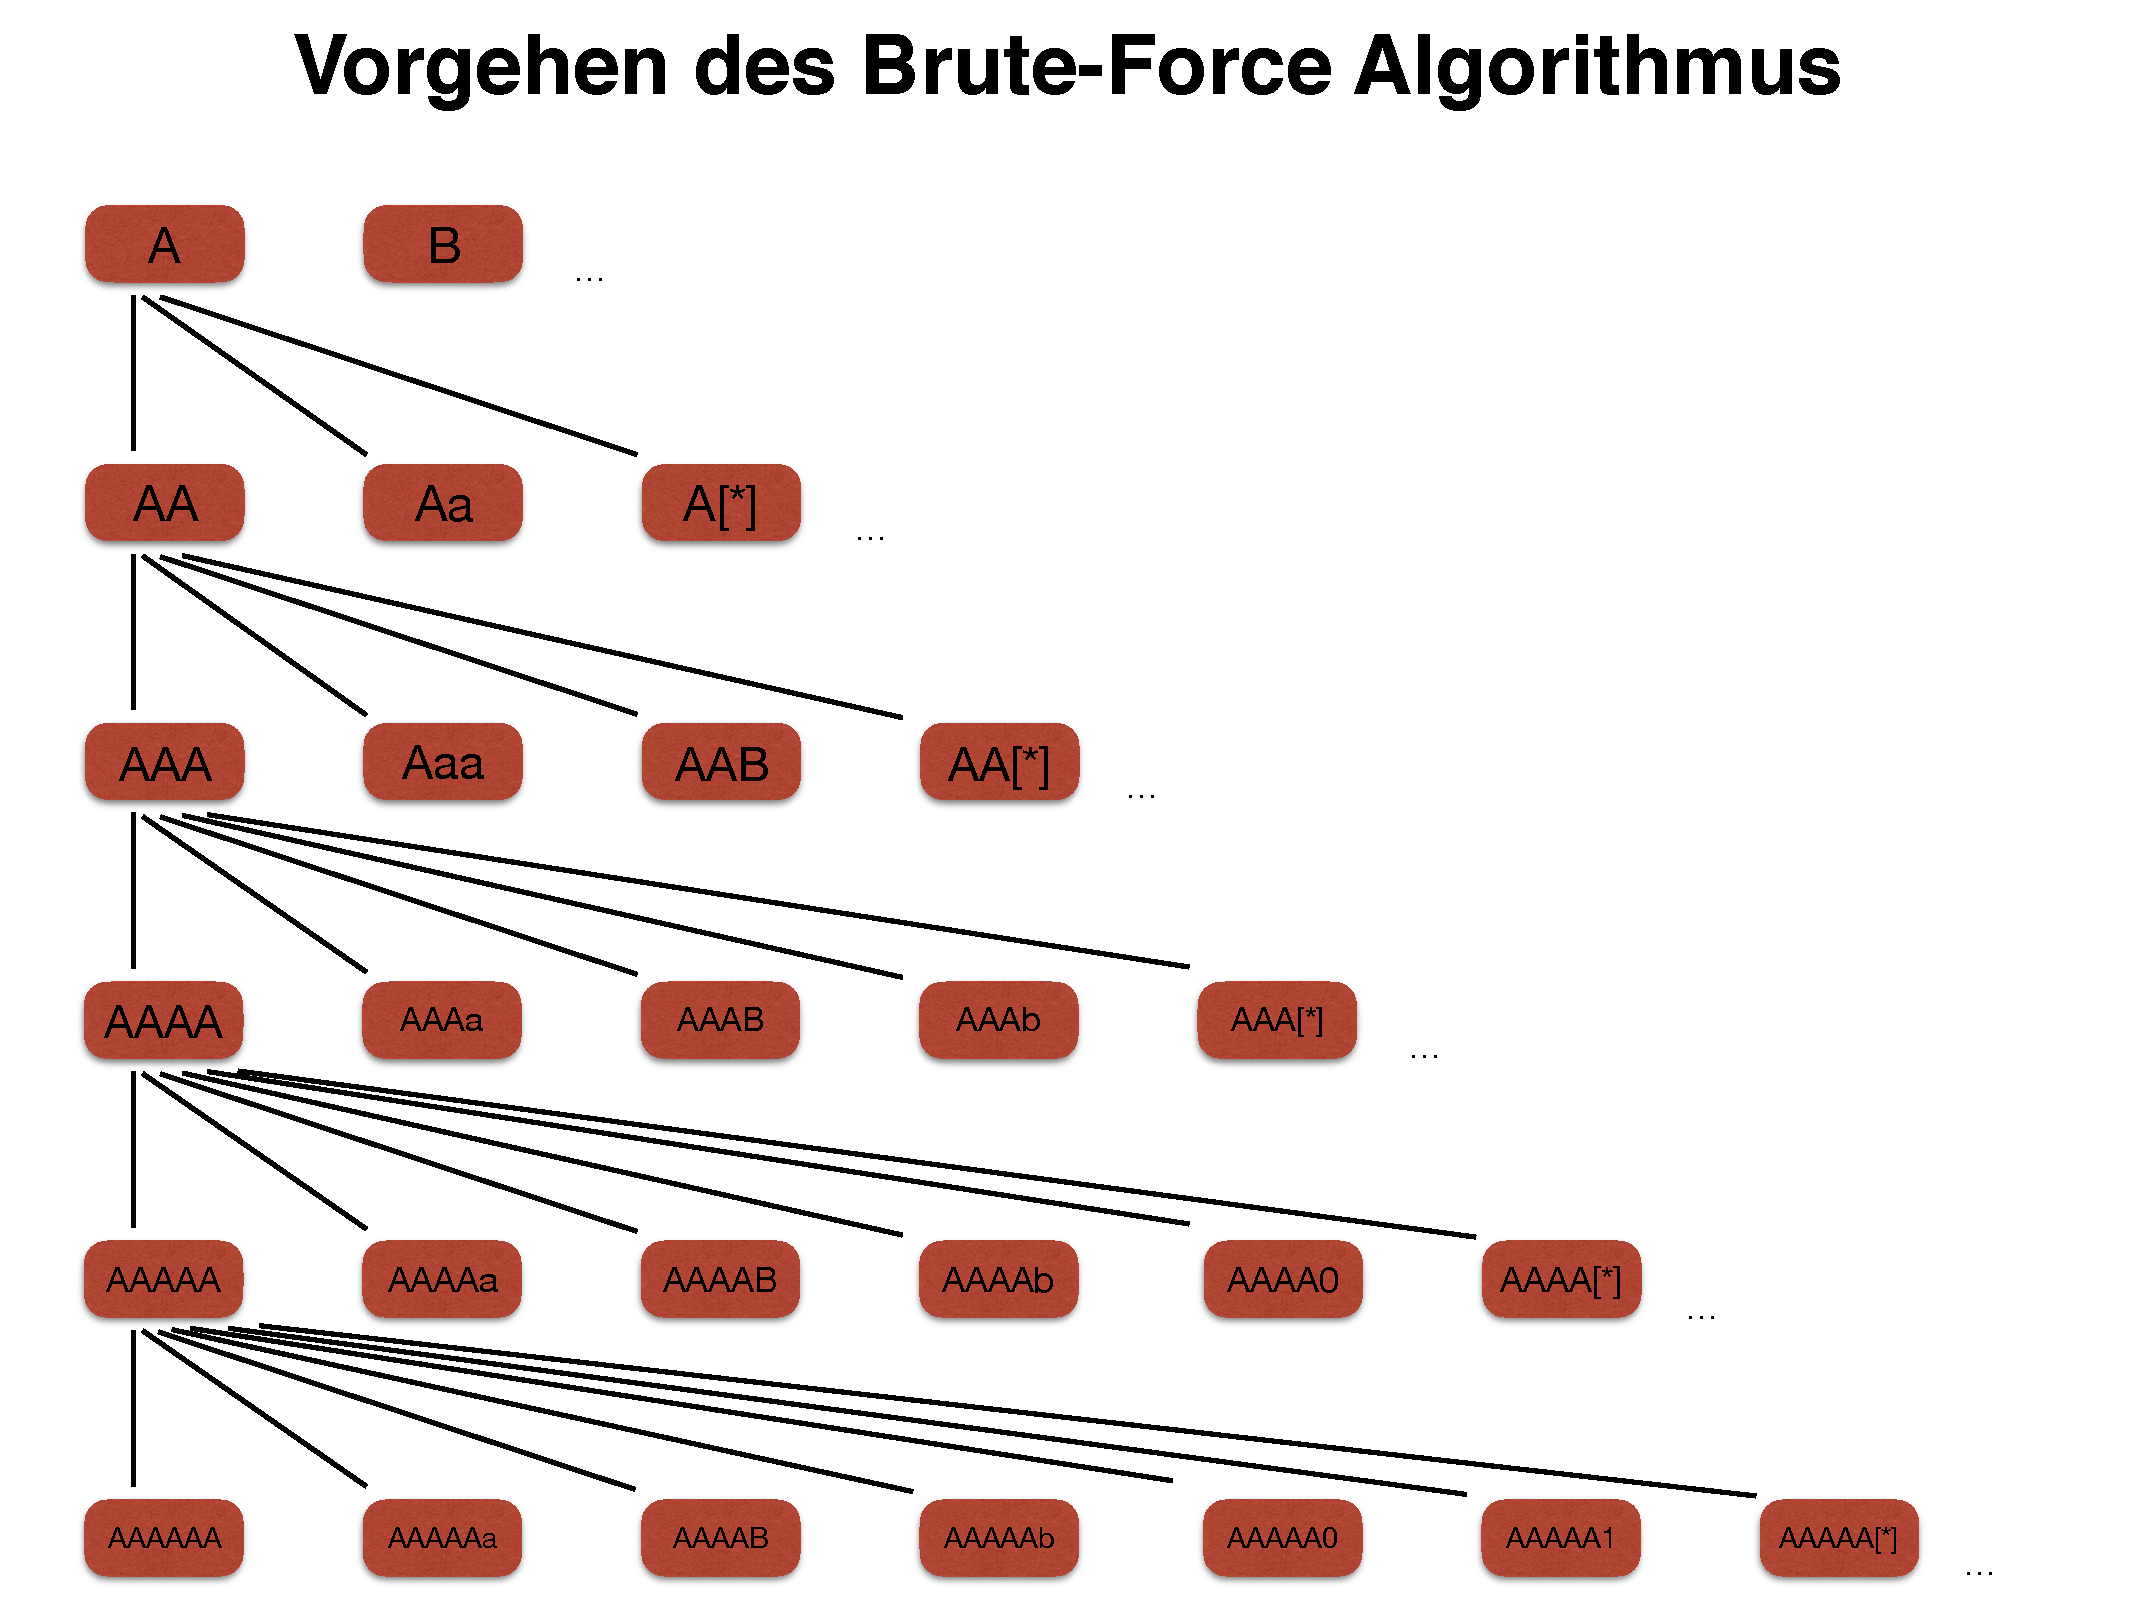
\includegraphics[natwidth=1200pt, natheight=349pt, width=1.0\textwidth]{images/SchaubildAlgorithmBreitensuche.pdf}
	\caption{Darstellung der Suchstrategie, die der Brute-Force Algorithmus zum Ermitteln des Passwortes benutzt.}
	\label{fig:schemaBruteForce}
\end{figure}

Die berechneten Passwörter werden dann in eine Warteschlange geschrieben, sodass sich die Worker des verteilten Systems (Beschreibung siehe \ref{glossar}) \enquote{Arbeitspakete} beziehen können. Ein solches Arbeitspaket beinhaltet eine Sammlung von Passwörtern. Die Worker berechnen dann die Hashes der Passwörter und vergleichen diese mit dem Zielhash.\\
 Berechnet ein Worker einen Hash, der mit dem Zielhash überein stimmt, so ist das gesuchte Passwort identifiziert.  

\newpage

\section{Architektur des verteilten Systems}
Das verteilte System wird so konzipiert, dass die vier in Kapitel \ref{allgemeineAnforderungen} genannten Anforderungen umgesetzt werden können. Um dies zu realisieren, wird mit einer nachrichtenbasierten Architektur geplant. Die Rechner des verteilten Systems können so miteinander kommunizieren, ohne dass eine restriktive Anordnung notwendig ist. Dadurch wird die Skalierbarkeit sichergestellt. \\
Außerdem realisiert die nachrichtenbasierte Architektur, dass die Ressourcen innerhalb des verteilten Systems leicht verfügbar sind. \\
Im verteilten System übernimmt der Master die Verantwortlichkeit für die Kommunikation, sodass die Skalierbarkeit weiter verbessert wird. Es wird lediglich ein Master im System benötigt, die Menge der Worker ist irrelevant. Konkret wird der Master die Funktion des Webservers beinhalten, welcher für die Steuerung des Nachrichtenversands innerhalb des verteilten Systems verantwortlich ist. Die Verbindungen werden mit Hilfe von Websockets aufgebaut.\\
Die Nachrichten werden versandt und bei jedem Rechner lokal in einer Warteschlange (MessageQueue) gespeichert. Somit besteht für das gesamte verteilten Systems jederzeit Zugriff auf alle Nachrichten. Je nach Inhalt der Nachricht (z.B. \enquote{Nachricht an Worker}) wird entschieden, wer die jeweiligen Nachrichten erhalten oder verarbeiten soll. 

In den folgenden Skizzen sind die Planungen auf konzeptioneller Ebene zusammengefasst.

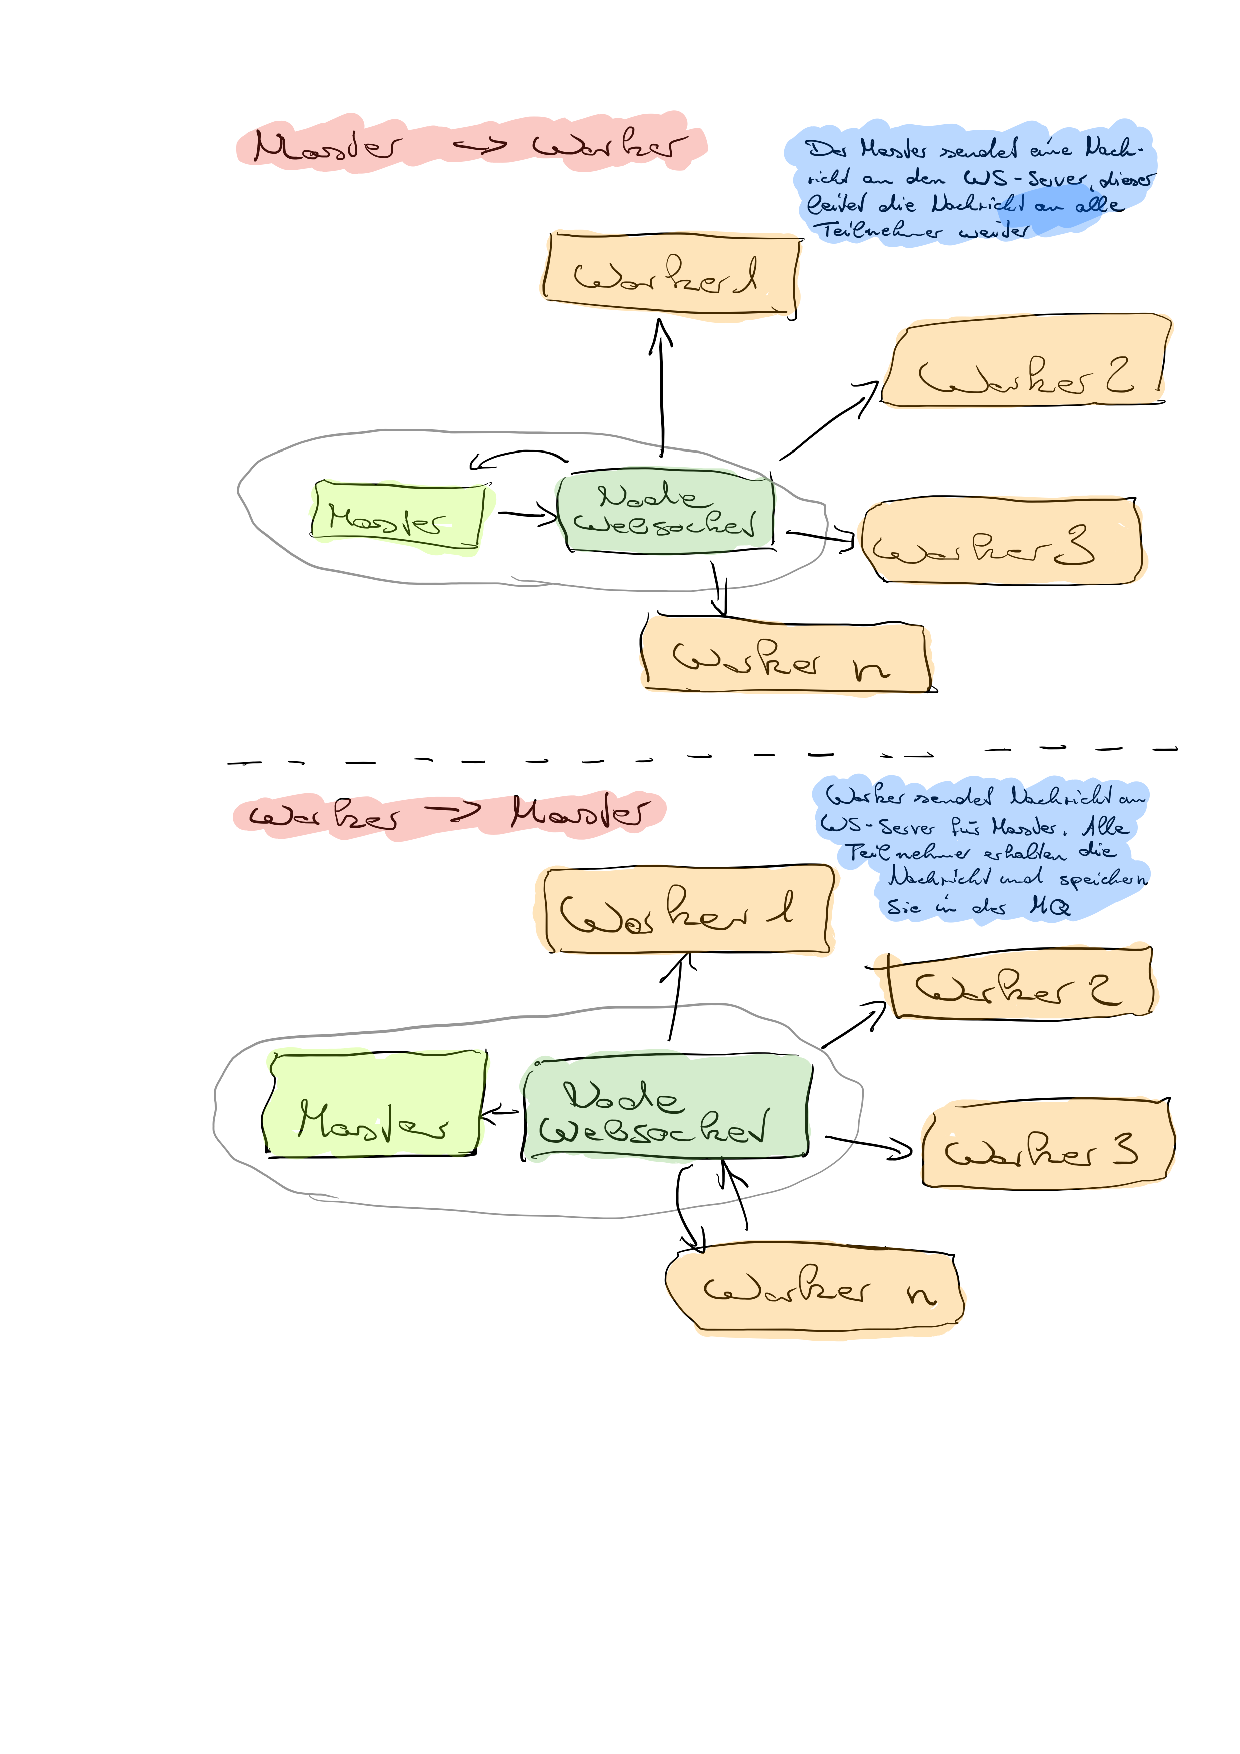
\includepdf[pages={1}]{images/systemarchitektur1.pdf}
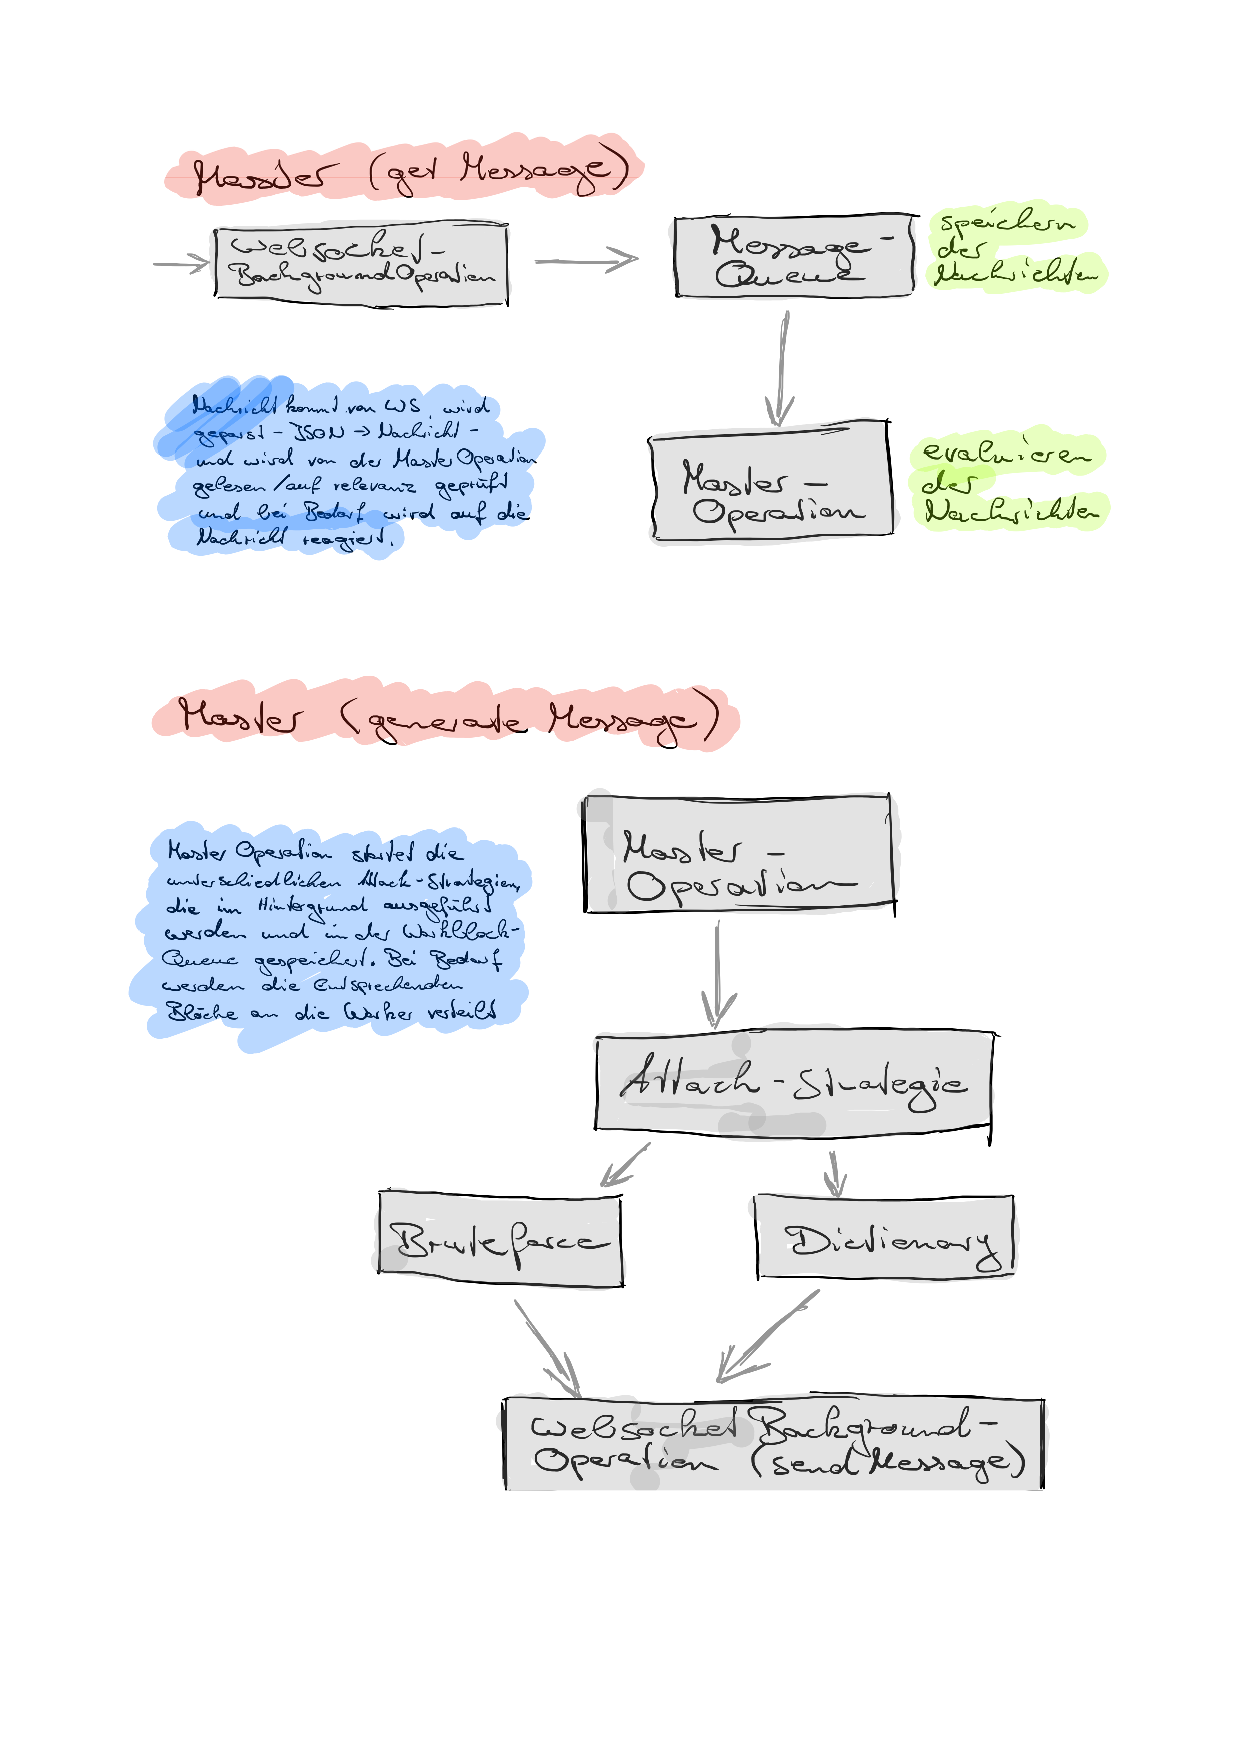
\includepdf[pages={1}]{images/systemarchitektur2.pdf}
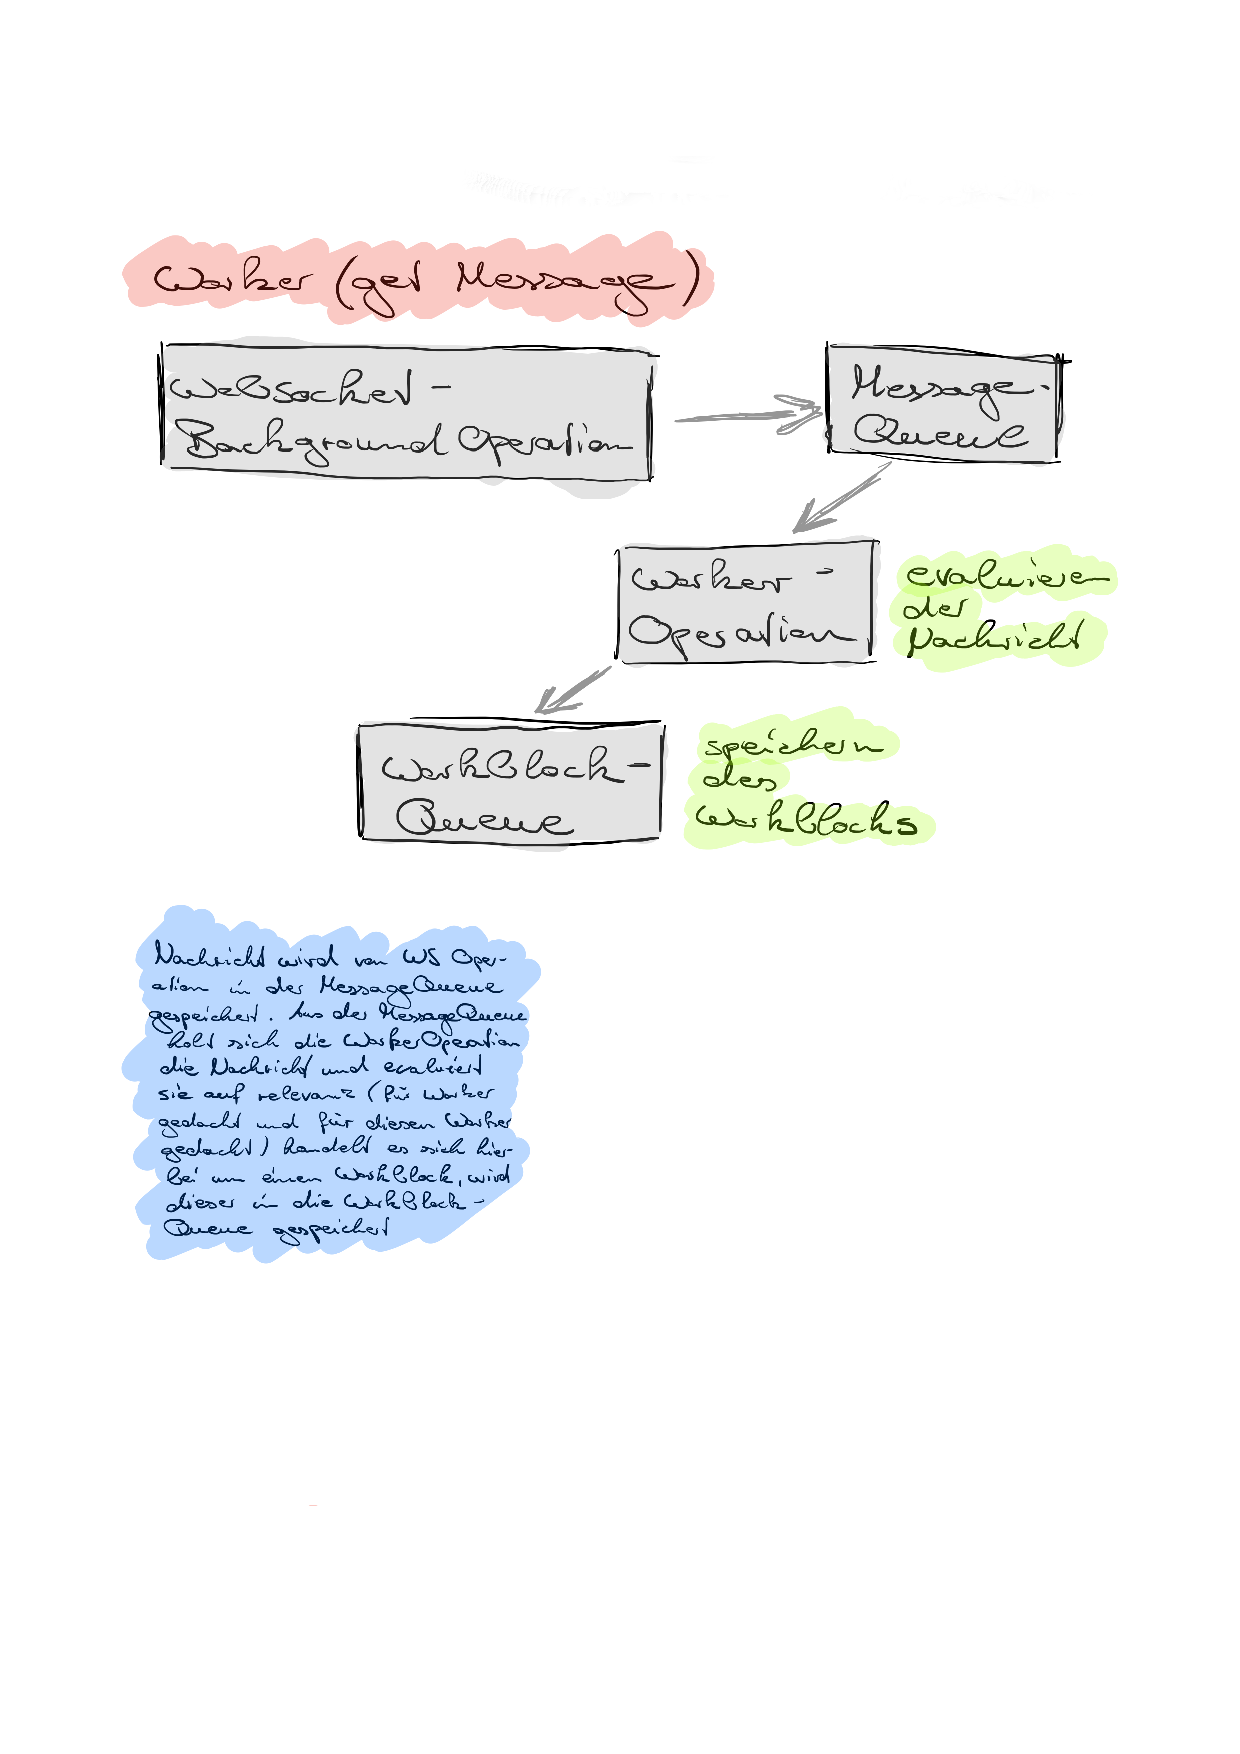
\includepdf[pages={1}]{images/systemarchitektur3.pdf}
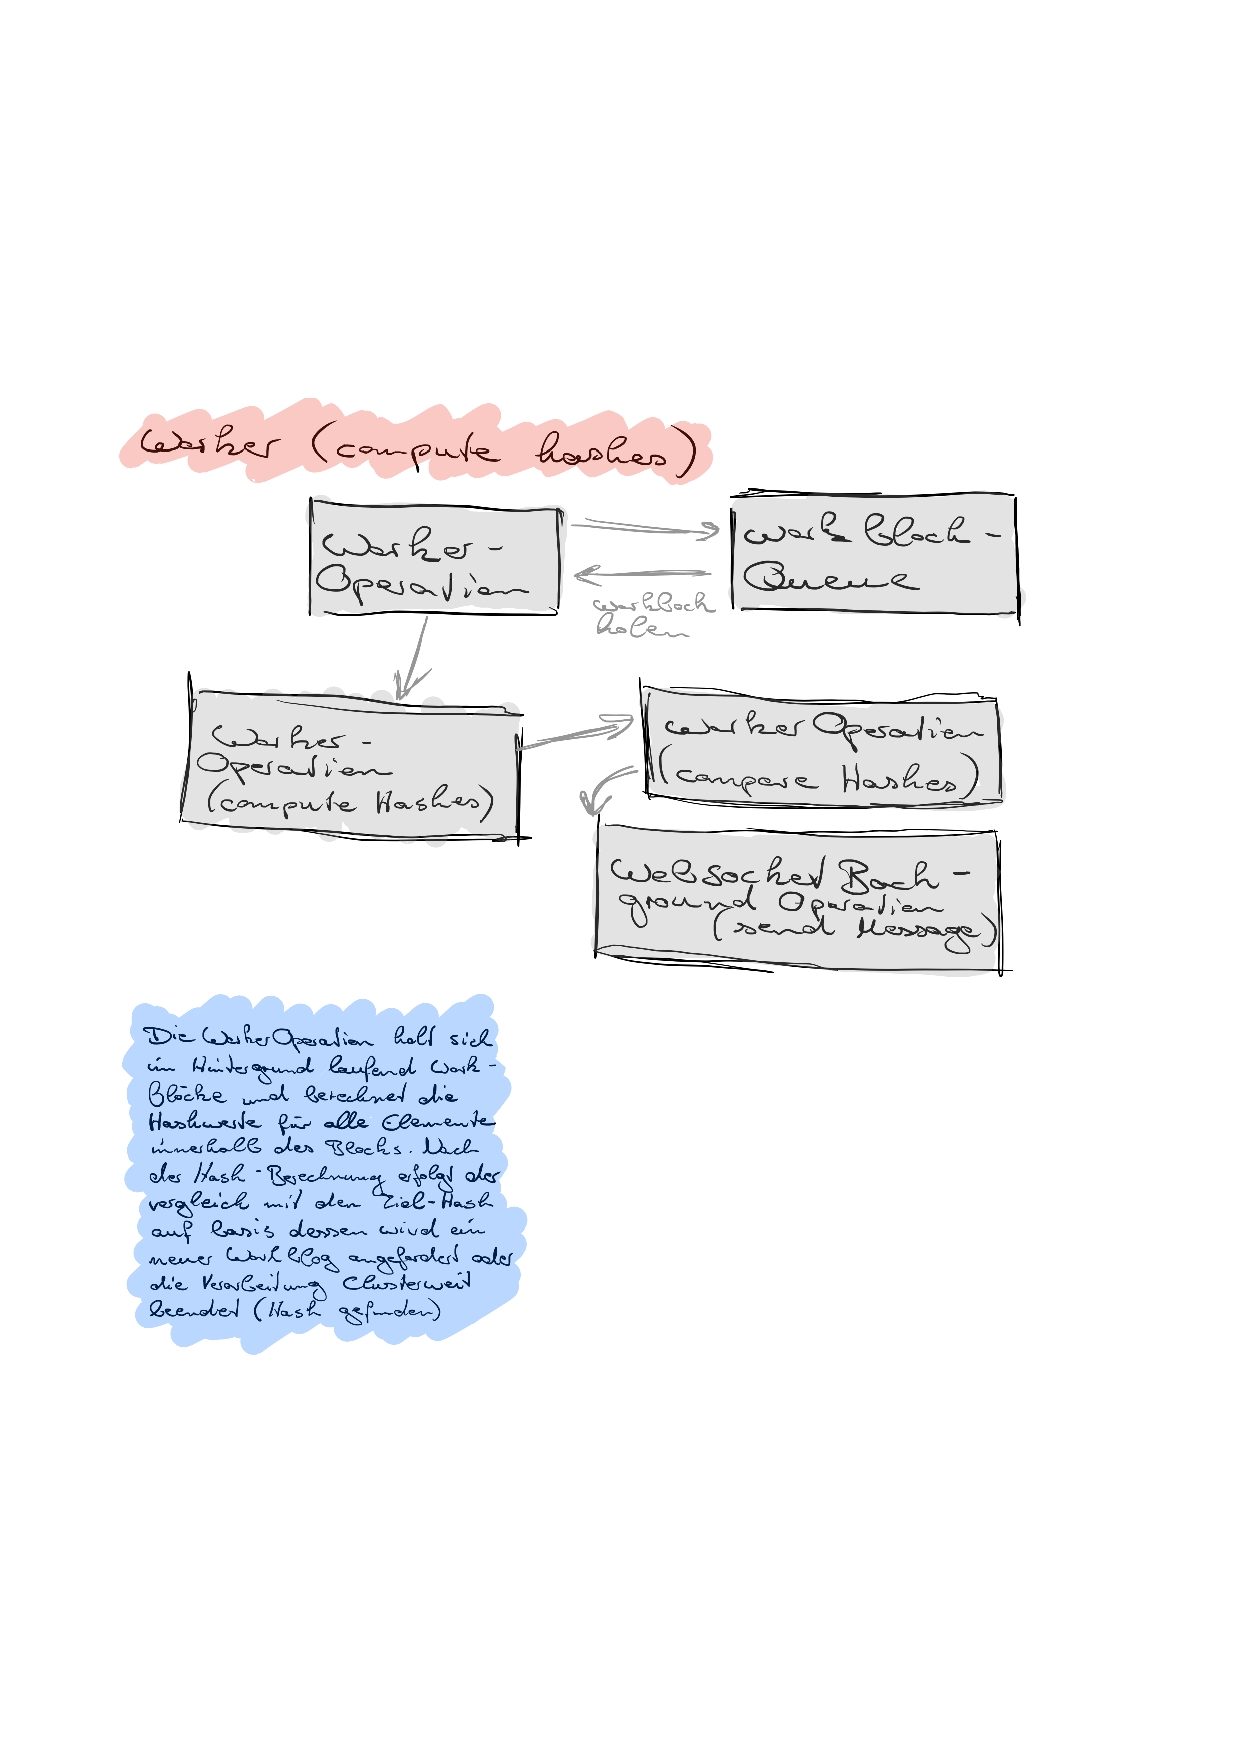
\includepdf[pages={1}]{images/systemarchitektur4.pdf}
 

\setcounter{table}{1}
\setcounter{figure}{1}
	\include{chapter/bruteForce} 

	
		\setcounter{table}{1}
\setcounter{figure}{1}
	\include{chapter/fazit} 

\singlespacing
 
  	%Erzeugt ein Abbildungsverzeichnis
	\listoffigures
	%Fügt die Zeile "`Abbildungsverzeichnis"' als Chapter ins Inhaltsverzeichnis ein
	\addcontentsline{toc}{chapter}{Abbildungsverzeichnis}
	
	%Erzeugt ein Tabellenverzeichnis
	\listoftables
	%Fügt die Zeile "`Tabellenverzeichnis"' als Chapter ins Inhaltsverzeichnis ein
	\addcontentsline{toc}{chapter}{Tabellenverzeichnis}
	
		
	%Ändert den Stil des Literaturverzeichnisses
	\bibliographystyle{geralpha}
	%Erzeugt das Literaturverzeichnis anhand der Datei "`literatur.bib"'
	\bibliography{literatur}
	%Fügt die Zeile "`Literaturverzeichnis"' als Chapter ins Inhaltsverzeichnis ein
	\addcontentsline{toc}{chapter}{Literaturverzeichnis}
  	


%=== Schlussteil =====================================================
% \backmatter
% \pagenumbering{Roman}

\setcounter{table}{1}
\setcounter{figure}{1}

\end{document}